\documentclass[10pt]{article}
\usepackage[margin=2.2cm]{geometry}
\usepackage{amsmath,amsthm}
\usepackage{newtxtext,newtxmath}
\usepackage{booktabs,graphicx,caption}
\usepackage[colorlinks=true,allcolors=blue!50!black]{hyperref}
\captionsetup{font=small}
\renewcommand{\thetable}{S\arabic{table}}
\renewcommand{\thefigure}{S\arabic{figure}}
\renewcommand{\thesection}{S\arabic{section}}
\usepackage{textcomp}
\IfFileExists{currency.tex}{\providecommand{\CurrencyName}{Chinese yuan}
\providecommand{\CurrencyCode}{CNY}
\providecommand{\CurrencySymbol}{\ifmmode\text{\textyen}\else \textyen\fi}
}{\providecommand{\CurrencyName}{Chinese yuan}
\providecommand{\CurrencyCode}{CNY}
\providecommand{\CurrencySymbol}{\ifmmode\text{\textyen}\else \textyen\fi}
}
\newcommand{\clipunit}{\operatorname{clip}_{[0,1]}}
\newcommand{\SLU}{1.27\times10^{8}}
\newcommand{\SLphi}{8.50}
\newcommand{\SLam}{1.33\times10^{9}}
\newcommand{\Srad}{6.05\times10^{-8}}
\newcommand{\Sbound}{2.74\times10^{14}}
\newcommand{\SgsMin}{356.20}
\newcommand{\SgsSweep}{1099}
\newcommand{\SgsFinal}{1063.82}
\newcommand{\SgsXa}{0.50}
\newcommand{\SgsXb}{0.37}
\newcommand{\SnMovers}{13}
\newcommand{\SstateTV}{19}
\newcommand{\SstateFlat}{27}


\title{Supplementary Material for ``Profit-Taking Strategies of Competing Virtual Power Plants Under Time-Variant Switching Costs: Equilibrium Analysis of a Multi-Leader--Multi-Follower Game''}
\date{}

\begin{document}
\maketitle
\vspace{-1.5em}
\noindent Equation, proposition, table, and figure numbers without the prefix ``S'' refer to the main text. The companion archive provides the data, code and independent equilibrium checks. The case studies report monetary amounts in \CurrencyName{} (\CurrencyCode{}, \CurrencySymbol{}).

\section{Physical Recruitment Mechanism}\label{sec:physical}
The two virtual power plants (VPPs), A and B, use Shapley allocation. Each fixed reference portfolio contains five distributed energy resources (DERs), comprising two renewable units (PV1 and PV2), a thermal generator (TG), an energy storage system (ESS), and a demand response (DR) unit. PV1 and PV2 are the manuscript labels for the wind and solar input series, respectively. B retains its full ESS capability. In portfolio A, ESS power takes the values $\beta=0.25,0.50,0.75,1.00$ times 1.50~MW. Energy capacity stays at 2~MWh, efficiency is fixed, and initial and final state of charge are both 0.50. The stand-alone value is recomputed at each power level. Each recruitment test adds a prospective copy of PV2 or of the ESS with the same parameters and input profiles as the original unit.

Increasing the storage power available to A raises the allocated increment $F$ of the prospective PV2 unit from $449.87$ to $511.67$, while its marginal contribution $s$ changes from $560.93$ to $562.44$. For the prospective ESS, $F$ falls from $1603.14$ to $1536.14$ and $s$ from $2034.13$ to $1995.23$ (Fig.~\ref{fig:physical}(a)). With B offering $x_{\mathrm B}=0.50$ and $\epsilon=0.10$, the highest ratio at which A attracts target DER~$e$ with probability one is $1-(0.50F_{e\mathrm B}+\epsilon)/F_{e\mathrm A}$ (Fig.~\ref{fig:physical}(b)).

At one-quarter ESS power, the largest ratios at which A secures PV2 and the additional ESS are approximately $0.43$ and $0.52$, respectively. A ratio of $0.50$ therefore attracts the prospective ESS with certainty, while A must offer PV2 a larger share of the increment to secure it. Increasing the power rating of A's current ESS raises the ratio A can quote to PV2 and lowers the one it can quote to the additional ESS. This comparison holds the background portfolios fixed and isolates the effect of storage power on offers. Copies of the same type use identical input profiles, and the market participation model omits network constraints, degradation, and demand rebound.

\begin{figure}[h]
\centering
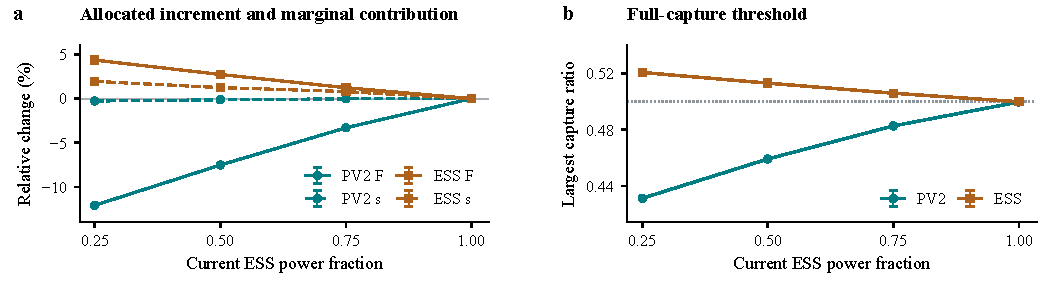
\includegraphics[width=\linewidth]{figs/physical_recruitment.pdf}
\caption{Physical recruitment. (a) Percentage change $100[z(\beta)/z(1)-1]$ for the target's allocated increment $F$ and marginal contribution $s$. In \CurrencySymbol{} per contract period, their full-power values are $(511.67,562.44)$ for PV2 and $(1536.14,1995.23)$ for ESS. (b) Largest ratio at which A attracts each target with probability one, for $x_{\mathrm B}=0.50$ and $\epsilon=0.10$. The reference line is $x_{\mathrm A}=0.50$.}
\label{fig:physical}
\end{figure}

\section{Positive Control}\label{sec:control}
The positive control has $F_{dv}=1$, $s_{dv}=0.20$, $A_v=1$, zero switching costs, and $\epsilon=0.30$. Against a rival ratio of $0.90$, the payoff of each virtual power plant operator (VPPO) is $2z$ for $0\le z\le0.60$ and $3z-5z^2/3$ for $0.60\le z\le1$. Both best responses are therefore $0.90$. From $(0.50,0.50)$, Algorithm~1 finds an approximate equilibrium at tolerance $\eta=2\times10^{-5}$. The ratios round to $(0.90,0.90)$, and an independent check gives maximum regret $1.95\times10^{-17}$ at the unrounded ratios.

\section{Twenty-DER Contracts}\label{sec:twenty}
Table~\ref{tab:twenty} lists the current members of each VPP and their remaining contract periods, drawn uniformly from $1,\ldots,L_v-1$. The independently refined quote rounds to $(0.03,0.20,0.00,0.19)$. At the unrounded quote, \SnMovers{} of the 20 DERs change VPP: all members of VPPs~1 and~3, DERs 12--14 of VPP~2, and DER~3 of VPP~4. VPP~2 gains ten of them, and DERs~12--14 join VPP~4. Every DER chooses its destination with probability one.

\begin{table}[h]
\centering
\caption{Current contracts at the twenty-DER switching window}
\label{tab:twenty}
\begin{tabular}{@{}cll@{}}
\toprule
VPP & Member indices $d$ & Remaining periods $r_d$\\
\midrule
1 & 6, 7, 8, 20 & 1, 1, 1, 1\\
2 & 1, 5, 12, 13, 14 & 2, 1, 1, 1, 1\\
3 & 4, 9, 15, 17, 18 & 3, 1, 2, 1, 2\\
4 & 2, 3, 10, 11, 16, 19 & 3, 1, 4, 4, 4, 4\\
\bottomrule
\end{tabular}
\end{table}

\section{Near-Zero Sensitivity Cases}\label{sec:nearzero}
Among the 2709 sensitivity configurations with a COPT quote within tolerance, 2694 also have a separately verified pure equilibrium with exactly zero regret. In the other 15 configurations, the COPT quotes have maximum regret at most $8.47\times10^{-7}$. An exhaustive test of the two-VPPO game excludes an exact pure equilibrium in each of these 15 configurations. Every candidate point and every profile on a candidate segment admits a profitable unilateral deviation.

\section{Best-Response Iteration in the Five-DER Case}\label{sec:gs}
Starting from $(0.50,0.50)$ in the five-DER baseline, the Gauss--Seidel best-response sequence did not converge over the observed trajectory. Its smallest maximum regret was $\SgsMin$ at a profile that rounds to $(\SgsXa,\SgsXb)$. The final profile had maximum regret $\SgsFinal$.

\section{Multi-Window Dynamics}\label{sec:dynamics}
The five-DER market starts from the five-DER baseline state in the main text with the equal propensity to disrupt method at VPP~1 and Shapley allocation at VPP~2, $L=(5,4)$, and $\epsilon=0.10$. At each window, the coefficients $F$, $s$, and $A$ are recomputed from coalition values for the current memberships. A member leaving early with $r_d>0$ pays the time-variant switching cost $C_d=\gamma_{o(d)}r_d$. Under the flat schedule it pays a fixed fee of \CurrencySymbol{}500. The rival deduction is $C_d/L_v$ and the incumbent's per-period compensation is $C_d/r_d$, which equals $\gamma_{o(d)}$ under the time-variant schedule.

At each window, the VPPOs use Algorithm~1 to select their posted ratios by minimizing maximum regret for the current contract state. The posted ratios meet the acceptance threshold when their verified maximum regret satisfies $\rho\le\eta-\delta$, with $\eta=10^{-3}$ and $\delta=10^{-6}$, both in \CurrencySymbol{} per contract period. Each DER then chooses a VPP independently according to the probabilities in equation~(17). The expectations include every affiliation outcome with positive probability. A member who switches or whose contract has expired starts a new contract of its VPP's length. Other members' terms fall by one. In the realized coalition, VPPO~$v$ receives $x_v I_{\mathcal S_v'}$ plus the payments it receives from members leaving early, and DER~$d$ receives $(1-x_v)$ times its allocated increment in the realized coalition, minus $C_d$ if it leaves early. A VPP with a single member offers that member a zero increment, and an empty VPP offers zero to all DERs.

Table~\ref{tab:dynamics} reports the expectations per window. In the more probable branch under time-variant switching costs, the ESS stays with VPP~1 in window~1, PV2 joins VPP~1 in window~2, and the DR unit follows in window~5. VPP~2 is then empty and VPPO~1 retains at least $99.95\%$ of its coalition surplus. In the other branch, the ESS joins VPP~2 and the posted quote exceeds the regret threshold in every window.

\begin{table}[h]
\centering
\caption{Five-DER outcomes per window. $P_\eta=\Pr(\rho\le\eta-\delta)$ is the probability of meeting the regret threshold, and $\mathbb E\rho$ is expected maximum regret. Regret, cash and DER gain are in \CurrencySymbol{} per contract period. Cash is the expected VPPO cash flow. DER gain is expected realized gain above stand-alone profit net of time-variant or flat switching costs. The Switches column gives the expected number of DERs that change VPPs, and $P_{\text{empty}}$ is the probability of an empty VPP.}
\label{tab:dynamics}
\small
\begin{tabular}{@{}rrrrrrrrrr@{}}
\toprule
Window & $P_\eta$ & $\mathbb E\rho$ & $\mathbb E x_1$ & $\mathbb E x_2$ & Cash$_1$ & Cash$_2$ & DER gain & Switches & $P_{\text{empty}}$\\
\midrule
\multicolumn{10}{@{}l}{\emph{Time-variant switching cost $\gamma_{o(d)}r_d$}}\\
1 & 0.00 & 160.84 & 0.50 & 0.11 & 1880.31 & 89.16 & 2540.52 & 0.19 & 0.00\\
2 & 0.81 & 46.50 & 0.42 & 0.10 & 1825.80 & 572.40 & 2209.14 & 1.19 & 0.00\\
3 & 0.81 & 35.19 & 0.57 & 0.10 & 2620.29 & 209.09 & 1580.74 & 0.58 & 0.00\\
4 & 0.81 & 78.73 & 0.57 & 0.11 & 2647.19 & 398.44 & 1561.72 & 0.58 & 0.00\\
5 & 0.81 & 45.68 & 0.53 & 0.10 & 2445.17 & 566.27 & 1780.71 & 1.19 & 0.00\\
6 & 0.81 & 44.49 & 0.90 & 0.09 & 4310.90 & 353.95 & 128.21 & 0.39 & 0.81\\
7 & 0.81 & 27.36 & 0.89 & 0.09 & 4340.79 & 252.49 & 2.56 & 0.58 & 0.81\\
8 & 0.81 & 59.98 & 0.90 & 0.10 & 4453.47 & 369.11 & -29.52 & 0.58 & 0.81\\
9 & 0.81 & 45.68 & 0.91 & 0.10 & 4327.67 & 364.42 & 100.06 & 0.39 & 0.81\\
10 & 0.81 & 44.49 & 0.90 & 0.09 & 4309.00 & 353.95 & 130.10 & 0.39 & 0.81\\
\multicolumn{10}{@{}l}{\emph{Flat switching cost 500}}\\
1 & 0.00 & 153.11 & 0.54 & 0.11 & 2058.06 & 96.89 & 2339.16 & 0.25 & 0.00\\
2 & 0.00 & 173.57 & 0.37 & 0.13 & 1520.72 & 802.69 & 2261.87 & 1.25 & 0.00\\
3 & 0.75 & 52.07 & 0.59 & 0.12 & 2540.25 & 326.58 & 1632.07 & 0.58 & 0.00\\
4 & 0.75 & 81.75 & 0.58 & 0.14 & 2534.74 & 433.20 & 1617.35 & 0.58 & 0.00\\
5 & 0.75 & 77.08 & 0.52 & 0.17 & 2321.96 & 791.99 & 1643.51 & 1.25 & 0.00\\
6 & 0.75 & 68.09 & 0.88 & 0.13 & 4087.17 & 421.56 & 249.89 & 0.49 & 0.75\\
7 & 0.75 & 60.56 & 0.89 & 0.12 & 4124.22 & 356.65 & 220.28 & 0.55 & 0.75\\
8 & 0.75 & 72.21 & 0.88 & 0.13 & 4107.46 & 423.69 & 227.48 & 0.55 & 0.75\\
9 & 0.75 & 77.08 & 0.88 & 0.13 & 4091.09 & 415.22 & 251.16 & 0.49 & 0.75\\
10 & 0.75 & 68.09 & 0.88 & 0.13 & 4085.40 & 421.56 & 251.66 & 0.49 & 0.75\\
\bottomrule
\end{tabular}

\end{table}

\section{Common Ratios and Large Response Parameters}\label{sec:grids}
Table~\ref{tab:grids} gives the maximum regret of every common ratio $x_v=c$ on a $0.05$ grid, with each VPPO deviating over $[0,1]$. The best grid point has regret $433.20$ at $c=0.60$ for five DERs and $1519.12$ at $c=0.35$ for twenty DERs. The corresponding regrets at the refined five- and twenty-DER profiles are $160.84$ and $98.41$, respectively. Table~\ref{tab:epsilon} gives the five-DER baseline results at $\epsilon=100$ and $1000$. At $\epsilon=1000$, an exact rational witness gives zero regret.

\begin{table}[h]
\centering
\caption{Maximum regret (\CurrencySymbol{} per contract period) at common ratios}
\label{tab:grids}
\small
\begin{tabular}{@{}rrr@{}}
\toprule
Common ratio $c$ & Five DERs & Twenty DERs\\
\midrule
0.00 & 1766.06 & 2780.24\\
0.05 & 1654.97 & 2306.30\\
0.10 & 1543.89 & 2019.36\\
0.15 & 1432.80 & 1732.42\\
0.20 & 1321.72 & 1551.93\\
0.25 & 1210.64 & 1617.29\\
0.30 & 1099.55 & 1610.26\\
0.35 & 988.47 & 1523.23\\
0.40 & 877.38 & 2298.31\\
0.45 & 766.30 & 3625.36\\
0.50 & 655.21 & 4952.42\\
0.55 & 544.13 & 6224.75\\
0.60 & 433.05 & 7498.93\\
0.65 & 695.23 & 8836.19\\
0.70 & 789.12 & 10441.14\\
0.75 & 1124.94 & 10568.26\\
0.80 & 1460.77 & 11753.18\\
0.85 & 1796.59 & 13006.93\\
0.90 & 2132.42 & 14564.58\\
0.95 & 2468.24 & 16734.67\\
1.00 & 2804.07 & 18087.55\\
\bottomrule
\end{tabular}

\end{table}

\begin{table}[h]
\centering
\caption{Algorithm~1 on the five-DER baseline at large response parameters. The bracket bounds minimum maximum regret in \CurrencySymbol{} per contract period. The decisions and affiliation probabilities $y_{d1}$ for VPP~1 use the unrounded quotes.}
\label{tab:epsilon}
\small
\begin{tabular}{@{}rllll@{}}
\toprule
$\epsilon$ & Decision & Bracket & Quote & $y_{d1}$ (PV1; PV2; TG; ESS; DR)\\
\midrule
100 & numerical exclusion & $[25.47,360.31]$ & $(0.64,0.44)$ & 1.00; 0.23; 1.00; 0.97; 0.00\\
1000 & approximate equilibrium & $[0.00,1.99\times10^{-22}]$ & $(0.76,0.75)$ & 0.68; 0.48; 0.60; 0.60; 0.47\\
\bottomrule
\end{tabular}

\end{table}

\end{document}
